% vim:ts=4:sw=4
%
% Copyright (c) 2008-2009 solvethis
% Copyright (c) 2010-2012 Casper Ti. Vector
% Public domain.

\chapter{The RCBHT}\label{sec:RCBHT}

%--------------------------------------------------------------------------------------------------------------------------------------------------

% Overview

The hierarchical taxonomy's goal was to connect human apropos actions like: ``approaching", ``rotating", ``aligning", ``snapped", and ``mated" with LLB's in a context-sensitive manner. One of the main challenges encountered in interpreting force signals is their inherent noise and spatio-temporal complexity. However, the force signals do inherently possess characteristics that describe the task at hand. The authors hypothesized that such characteristics could be extracted by looking at how temporal relative changes were associated to each other and contextualized by the state in which they occur. In so doing, intuitive behavior sequence's can be extracted and their outcome examined. This level of discrimination is significant as it can be expanded to a real-time implementation and allow to reason about the state to perform corrective motions if necessary.
To bootstrap the approach, we partitioned the data into linear segments that approximate the data and classify the gradients according to magnitude per a small set of criteria. The next layer of abstraction examines at ordered-pair primitive sequences, and according to the gradient patterns presented and a small set of classification criteria, they are categorized into one of several types of motion compositions. The third layer abstracts sequences of motion compositions to identify LLB's, while the fourth layer looks at what LLB's are present in which states to determine if desired high-level behaviors are present. The final layer outputs the verification process results' according to whether or not the desired sequence of HLB's is present or not. A visualization of the hierarchical taxonomy can be seen in Fig. \ref{fig:Taxonomy}.
%--------------------------------------------------------------------------------------------------------------------------------------------------
\begin{figure}[h]
    \centering
    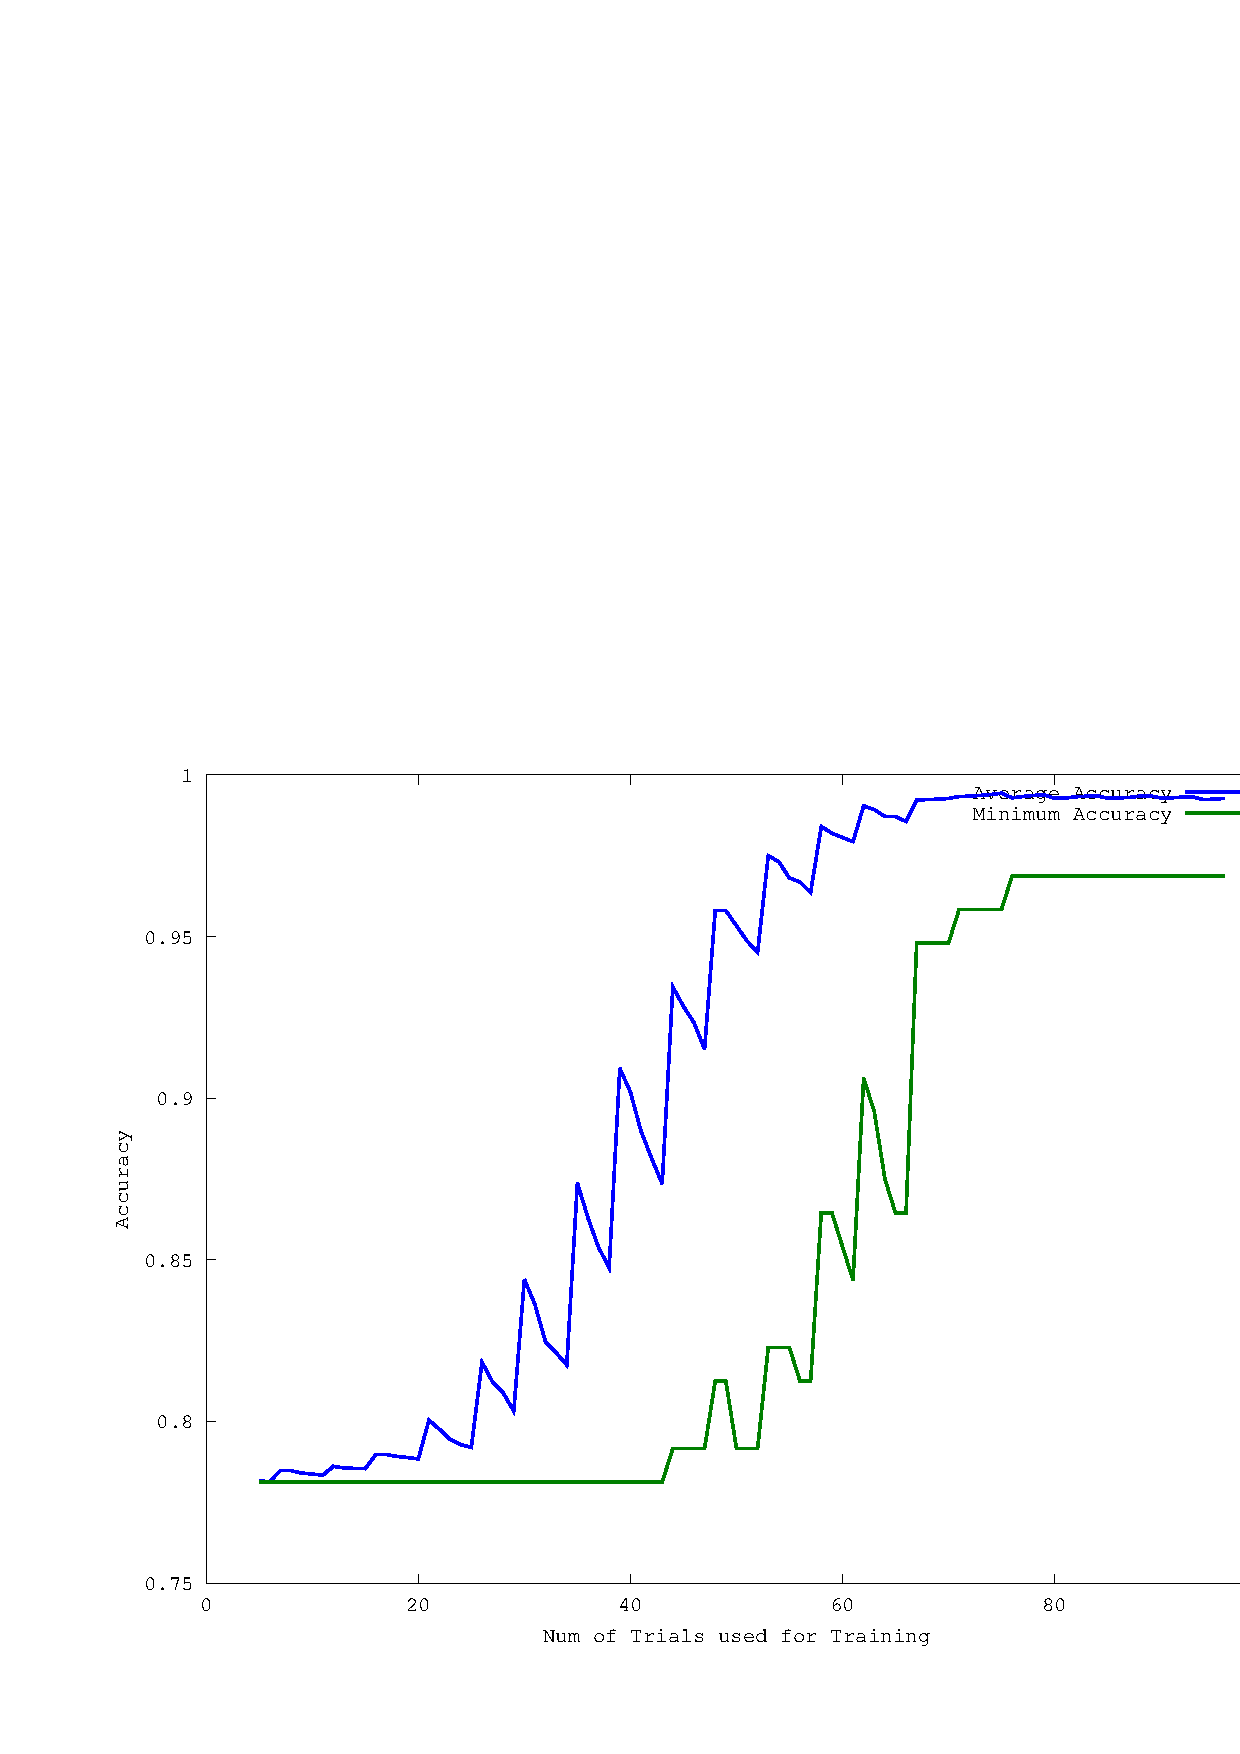
\includegraphics[width=3.35in, height=2.5in]{./img/encl2/2.png}
    \caption{The Relative Change-Based Hierarchical Taxonomy (RCBHT) for Cantilever-Snap Assembly Verification.}
    \label{fig:Taxonomy}
\end{figure}
%--------------------------------------------------------------------------------------------------------------------------------------------------
%--------------------------------------------------------------------------------------------------------------------------------------------------
\section{Primitive Layer} \label{subsec:Primitives}
%--------------------------------------------------------------------------------------------------------------------------------------------------
% Primitives: Signal Approximation through linear fits + Gradient + Data Structure
The primitives layer requires that each signal is partitioned into linear segments of data that closely approximate the original signal. Linear regression in concert with a correlation measure (the determination coefficient $R^2$) is used to partition the data whenever a minimum correlation threshold is crossed. If the determination coefficient drops under a given threshold the linear fit is partitioned and a new regression is started. The $R^2$ coefficient is a correlation measure that studies the ratio of the sum of the squares of the residual errors between the original data $y$ and the fit data $\hat{y}$ to the sum of the variance $\sigma{_y}^2$ as shown in Eqtn. \ref{eqtn:DeterminationCoefficient}.
%--------------------------------------------------------------------------------------------------------------------------------------------------
\begin{equation}
\label{eqtn:DeterminationCoefficient}
    R^2 = 1 - \frac{\sum{(y-\hat{y})^2}}{\sigma{_y}^2}
\end{equation}
%--------------------------------------------------------------------------------------------------------------------------------------------------
The threshold used to partition the data was set at 0.70, such that if the correlation dropped to under $70\%$, a linear segment or ``partition" would be generated, and a new one would start at the next data point. The data was traversed by a window equal to five data points (the data was sampled at a frequency of 1kHz by the simulation). The threshold values and the window length were empirically selected to partition the data sufficiently to capture relevant changes in the signals.
Each partition was accompanied by a data structure with seven types of information about itself: the average value across data points, the maximum value, the minimum value, the start time, the end time, the gradient value, and a gradient label. With respect to the latter, nine gradient labels (positive impulse, `pimp'; big, medium, and small positive gradients, `b/m/spos'; constant gradients, `const'; and their negative equivalents, `nimp', `b/m/s/neg') were assigned according to ranges summarized in Fig. \ref{tbl:GradientRangeValues}.
%--------------------------------------------------------------------------------------------------------------------------------------------------
\begin{figure}[h]
    \centering
    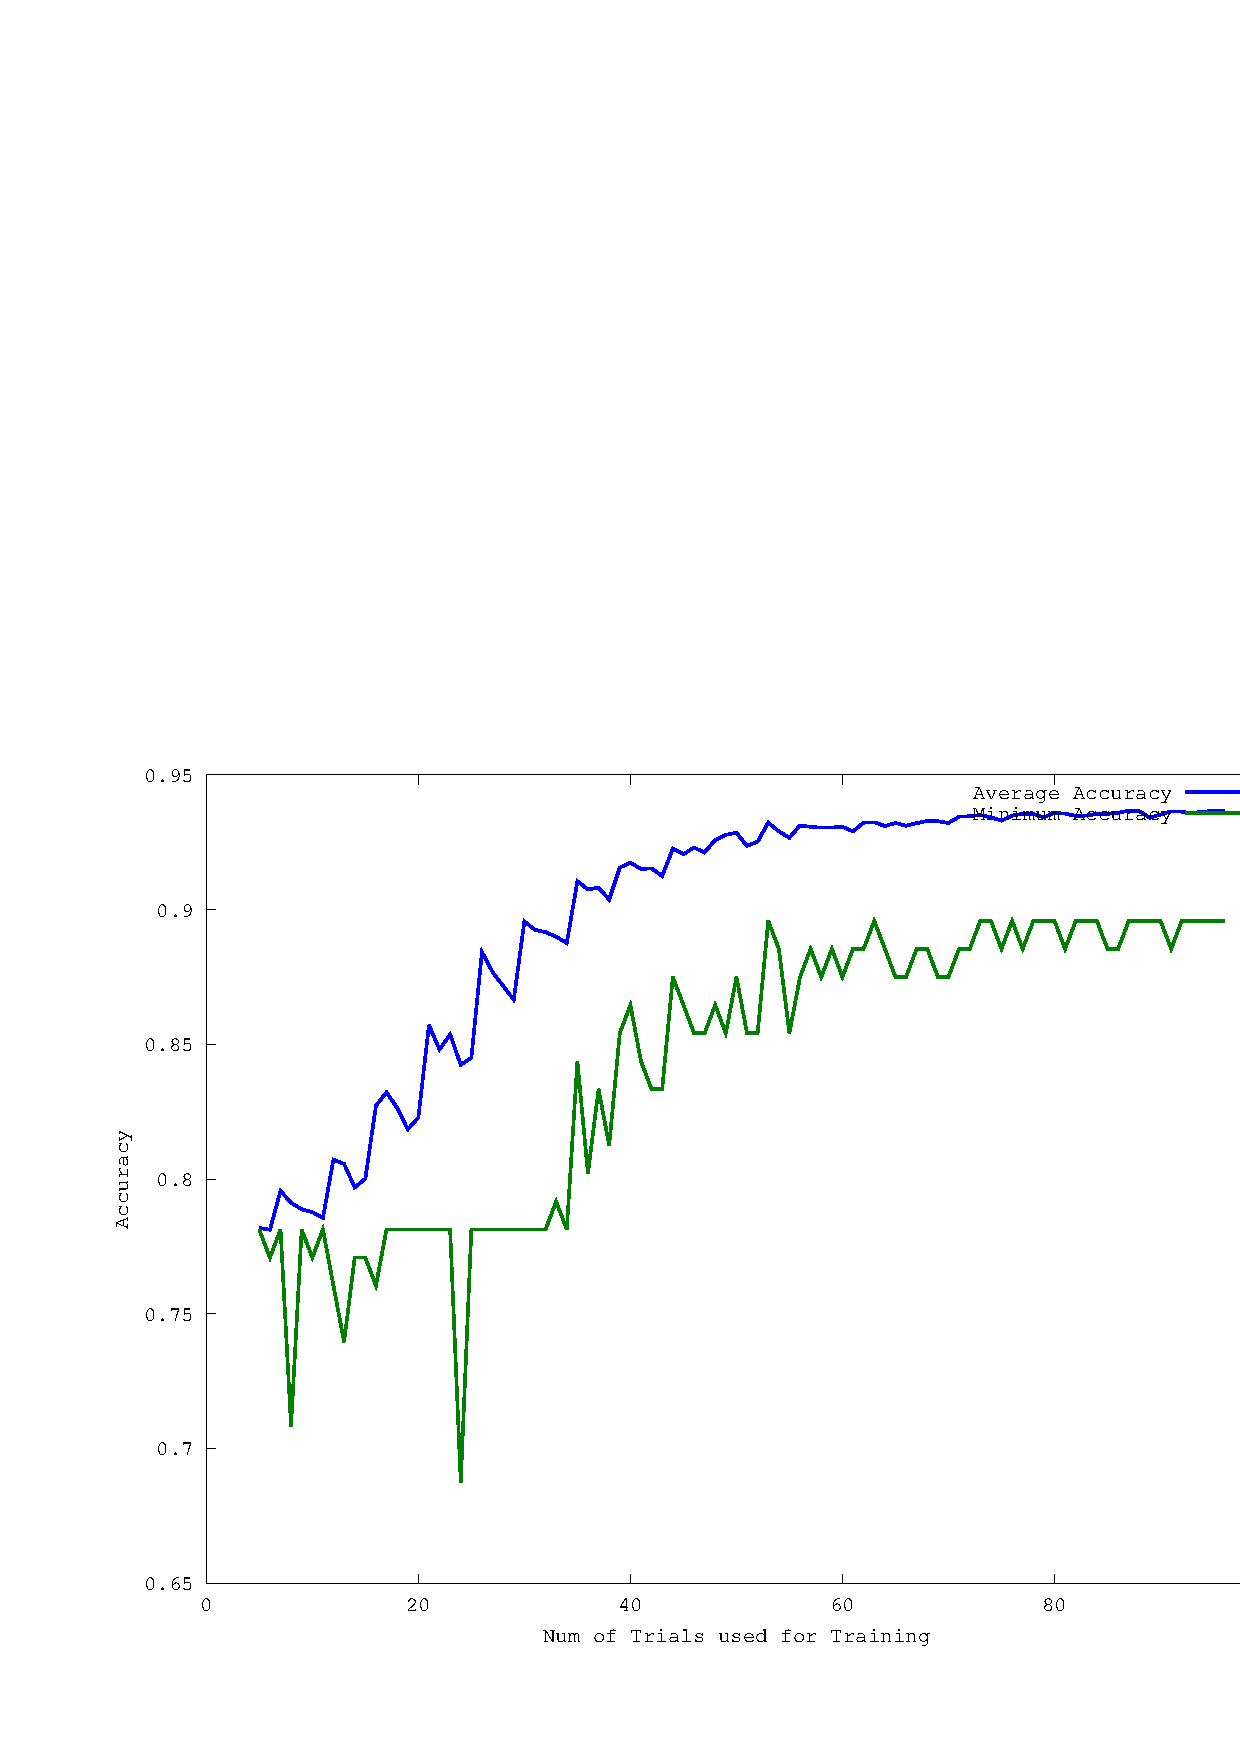
\includegraphics[width=2.75in,height=1.5in]{./img/encl2/3.png}
    \caption{Gradient values classification for the Primitives layers.}
    \label{tbl:GradientRangeValues}
\end{figure}
%--------------------------------------------------------------------------------------------------------------------------------------------------
The classification first attempts to separate instances of data in which contact or mating takes place. On the one hand, contact phenomena is characterized by very rapid and large changes in force signals, almost approximating an impulse. To this end, positive and negative impulses were categorized for gradients with values greater or less than 70. On the other hand, for mating situations, there is little or no change in force, for this reason a constant label was assigned to signals with gradient values less than the absolute value of 1. In between these two extremes we chose to have three gradient categories for both positive and negative signals to give a general idea of the magnitude change registered for a signal. Fig.\ref{fig:hlBehs} shows how the segmentation looks like across all five states (which are represented by five colored boxes) for the force signal in the x direction for PA10 related-experiments.
%--------------------------------------------------------------------------------------------------------------------------------------------------
%\begin{figure}[p!]
%    \centering
%        \includegraphics[width=4.50in, height=1.75in]{../../templates/figures/2012/IROS/PrimitivesFx.eps}
%        \caption{Primitive Layer: each red line represents a primitive that approximates the original signal.}
%        \label{fig:Primitives}
%\end{figure}
%--------------------------------------------------------------------------------------------------------------------------------------------------
%--------------------------------------------------------------------------------------------------------------------------------------------------
\section{Composites} \label{subsec:Composites}
%--------------------------------------------------------------------------------------------------------------------------------------------------
% Composites: Combinations of primitives
The next layer of abstraction identifies seven basic motions compositions (MC) by looking at ordered-pair sequences of primitives. The MC layer set is comprised of: adjustment, increase, decrease, constant, contact, positive contact, negative contact, and unstable motions. The positive and negative contacts, imply the sign of the (gradient) of the action.
A protocol was followed to minimize the effects of noise or erroneous segmentation. With respect to adjustments, primitives with big-to-small positive or negative gradients were considered as a positive or negative primitive category respectively. If a positive grouped primitive was followed by a negative grouped primitive an adjustment classification would be assigned to the ordered pair. Adjustments are motions in which the wrist records a quick `back-and-forth" motion typically seen during alignment or insertion operations as the force controller tries to minimize residual errors. The reason to group positive and negative gradients is to maximize the likelihood of group adjustments even when the rate of change may be slightly different. Furthermore, for this particular category, we used a window of two data points instead of one to look for a matching pair (all other categories looked at the contiguous primitive). That is, if after finding a positive or negative gradient, and if the next data point was not negative or positive respectively, we would look at the next data point to look for a pair. Such procedure mitigates the presence of spurious signals that could prevent the proper grouping of an adjustment movement.
The ordered pair groupings for motion composition classification are summarized in Fig. \ref{fig:MotionCompositions}. Note that the table contains sub-tables representing eight possible motion composition classifications. Each of which can be comprised of different sets of primitive groupings as illustrated in Fig. \ref{fig:MotionCompositions}.
%--------------------------------------------------------------------------------------------------------------------------------------------------
\begin{figure}[h]
    \centering
    \includegraphics[height=1.5in,width=4in]{./img/encl2/4.png}
    \caption{Motion Compositions according to primitive pairs in any order.}
    \label{fig:MotionCompositions}
\end{figure}
%--------------------------------------------------------------------------------------------------------------------------------------------------
As with the primitives layer, 11 pieces of information were collected for each MC: composition label, average value, root means square value, amplitude, the labels of the first and second primitives, the starting and ending times for both primitives, and the average time for both primitives.
%--------------------------------------------------------------------------------------------------------------------------------------------------
\subsection{Refinement} \label{subsubsec:Refinement1}
%--------------------------------------------------------------------------------------------------------------------------------------------------
After the MCs are generated, a refinement phase was used to filter less significant signals and augment more significant signals. To do so, the compositions were analyzed under three contexts: (1) a composition's time duration, (2) a composition's amplitude magnitude, and (3) composition repetition patterns.\\
%--------------------------------------------------------------------------------------------------------------------------------------------------
- Time Duration Context: this filter examines two contiguous MCs. If either composition is seven times bigger than the other, the smaller composition is merged to the larger one and all data is updated correspondingly. The duration ratio was determined empirically.\\
- Amplitude Value Context: this filter pertains to the formation of adjustment signals and constant signals. We considered three possibilities:
(i) If there are contiguous primitives of types PC/NC or NC/PC, and if their amplitude is ten times smaller than the largest amplitude registered in the assembly, then treat them as an adjustment. This criteria seeks to disambiguate real contact signals and false ones by looking at their amplitude. Real contacts are characterized by large values.
(ii) Similarly, if their is either an increase followed by a decrease and vice-versa, and both compositions have a similar amplitude (within ($50\%$) of each other and they have a similar average value ($100\%$) of each other, then merge as an adjustment and update the data correspondingly.
(iii) If there is a sequence of an increase followed by a constant, or a decrease followed by a constant and vice-versa, and they have a similar amplitude ($150\%$)and similar average value ($100\%$), then merge them as a constant and update their information. This last filter targets small noisy signals that appear as increases or decreases but that in effect are constants. The amplitude threshold value is larger here to give more possibilities of catching increases or decreases within the narrow range of the constant's amplitude.
- Repeated Compositions: the last filter takes signals that repeat and merges them as one. This filter is run iteratively until no more repetitions occur in the data.\\
%--------------------------------------------------------------------------------------------------------------------------------------------------
The post-refinement composition layer results are shown in Fig. \ref{fig:hlBehs} for a force signal sample in a Pivot Approach trial.
%--------------------------------------------------------------------------------------------------------------------------------------------------
%\begin{figure}[p!]
%    \centering
%        \includegraphics[width=4.50in, height=1.75in]{../../templates/figures/2012/IROS/CompositesFx.eps}
%        \caption{Composites Layer: motion composites are generated from a sequence of primitives. Their labels are show above the signal.}
%        \label{fig:Composites}
%\end{figure}
%--------------------------------------------------------------------------------------------------------------------------------------------------
%--------------------------------------------------------------------------------------------------------------------------------------------------
\section{Low-Level Behaviors} \label{subsec:llbeh}
%--------------------------------------------------------------------------------------------------------------------------------------------------
% Low-Level Behaviors: Combinations of Composites
The taxonomy's third layer considers motion composition ordered pairs along with signal duration and amplitude to yield classifications. Eight LLB classifications were derived and labeled as: {push, 'PS'}, {pull, 'PS'}, {contact, 'CT'}, {fixed, 'FX'}, {alignment, 'ALIGN'}, {shift, 'SH'}, and {noise, 'N'}. The LLB formulation criteria is similar to those at the MC level. That is, for a pair of increase MCs labels, or decrease MCs labels, or constant MCs labels or adjust MCs labels; pull, push, fixed, or adjust LLBs are assigned respectively. As for contacts, if there is a positive contact followed by a negative one, or vice-versa, a contact LLB is assigned. One major difference between the MC level and the LLB level is introduction a shifting behavior `SH'. Shifts and alignments are similar but differ in that, whenever there are two contiguous adjustment compositions, if the second composite's amplitude is larger than the first, label it as `SH' LLB, if smaller label it `ALGN'.
With regards to the time duration context, if any motion composition lasts more that 100 milliseconds, it can by itself be a low-level behavior, or if the contiguous composition is of the same classification they can also merge correspondingly. If any composition is less than the allotted duration and it does not have a matching pair, it is considered a noisy signal. With regards to the amplitude context, if there are two adjustments within a window of 2 data points, and their amplitudes decrease, render such a pair as an alignment, otherwise consider it a shift (or growing de-alignment). As for paired increase, decreases, and constants, they will yield pull, push, and fixed low-level behaviors correspondingly. Finally, as for contacts, if there is a positive contact followed by a negative one, or vice-versa, or even a stand-alone contact motion primitive, render this is a low-level contact behavior.
%--------------------------------------------------------------------------------------------------------------------------------------------------
\subsection{Refinement} \label{subsubsec:Refinement2}
%--------------------------------------------------------------------------------------------------------------------------------------------------
The LLB layer is also followed by a refinement phase. The latter filters based on the same three contexts as used before:\\
- Time Context: this filter examines two contiguous behaviors (except for contacts). If either behavior is five times bigger than the other, then merge towards the longer behavior and update the data correspondingly. LLB's are longer than compositions, so this threshold value is to be smaller than the one used for the composition's time duration filtering. \\
- Amplitude Context: the amplitude context pertains to alignments and shifts and there are four possible scenarios: (i) If there is a push-pull pair in either order and they have similar amplitudes ($150\%$) and similar average values ($100\%$) render then an alignment. (ii) If there is a shift followed by an alignment, or an alignment followed by a shift, where the second behavior has a smaller amplitude, then merge these as an alignment. This kind of merging is interesting because it can only be seen at this level of abstraction. While there may be a contiguous alignment-shift pair that was irreconcilable earlier, it can now be identified as an alignment. The same is done for a shift. (iii) Finally if there is an alignment followed by a pull or push or viceversa and they have similar amplitude ($50\%$) and similar average value ($100\%$), then merge as an alignment. In this case, after the previous refinement steps have been executed, if there are outstanding alignment-push or -pull pairs, the second behavior is a considered a continuation of the alignment and is merged. Shifts are treated similarly.\\
- Repeated Behaviors: As in the compositions layer, any two repeated behaviors can be merged as one.
The post-refinement LLB layer is shown in Fig. \ref{fig:hlBehs} for a sample signal in the Pivot Approach.
%--------------------------------------------------------------------------------------------------------------------------------------------------
%\begin{figure}[p!]
%    \centering
%        \includegraphics[width=4.50in, height=1.75in]{../../templates/figures/2012/IROS/llBehFx.eps}
%        \caption{LLB Layer: behaviors in this layer are generated from a sequence of motion composites. Their labels are shown below the signal.}
%    \label{fig:llBehs}
%\end{figure}
%--------------------------------------------------------------------------------------------------------------------------------------------------
%--------------------------------------------------------------------------------------------------------------------------------------------------
\section{High-Level Behaviors}\label{subsec:hlbeh}
%--------------------------------------------------------------------------------------------------------------------------------------------------
% High-Level Behaviors: Contextual combinations of low-level behaviors
The fifth layer contextualizes the process monitoring by asking what low-level behaviors principally describe the high-level human apropos behaviors found in the Pivot Approach: Approach, Rotation, (Alignment), Snap Insertion, and Mating\footnote{In actuality, we do not directly assess the Approach stage given that there are no contact forces at this stage. But if the rotation analysis is successful we assume that the approach was too.}.
% Key combinations
Then, if key combinations of LLB's across the six force axes for a specific state are identified, then a certain HLB can be ascertained. For each state and corresponding HLB an LLB or sequence of LLB's are matched with a particular force axis as part of the selected criteria. The criteria is connected both to the PA states, to the Controller Templates, and to the coordinate frame assignments in local coordinates (see Fig. \ref{fig:PA10_ExperimentalSetup} and Fig. \ref{fig:HIRO_ExperimentalSetUp}). Given that we have two implementations of the PA and Controller templates for the PA10-Two Snaps configuration and the HIRO-Four Snaps configuration we have two sets of key LLB criteria. They are presented in Fig. \ref{fig:KeyLLBs}.
%--------------------------------------------------------------------------------------------------------------------------------------------------
%-----------------------------------------------------------------------------------------------------------------------------------------
\begin{figure}[h]
    \centering
%    \subfigure{\label{fig:PA10_KeyLLB}\includegraphics[height=1.25in,width=2.4in]{./img/encl2/4.png}}
%    \hspace{0.04cm}
    \label{fig:HIRO_KeyLLB}\includegraphics[height=1in,width=2.4in]{./img/encl2/5.png}
    \caption{Comparison of the LLBs for both the PA10 and HIRO experimental configurations.}
    \label{fig:KeyLLBs}
\end{figure}
%----------------------------------------------------------------------------------------------------------------------------------------
\subsection{Key LLB's for PA10-Two Snap Experimental Configuration}
%----------------------------------------------------------------------------------------------------------------------------------------
The reasoning behind the selection of LLB's and axis for the Pivot Approach is intuitive. In state 2, the Rotation state, the wrist maintains a constant force along the z-direction, while the force along the y-direction diminishes as the wrist aligns itself with male part. The rotation about the x-axis can be seen through a series of large alignments along the moment's x-direction. For state 3, all axes are aligning in some form. For force elements, there is an alignment in position, for moment elements there is an alignment in orientation. The only exception to this is the moment about the z-direction. A pattern emerges where the moment axis that corresponds to the wrist's direction of motion for the insertion (i.e. the z-axis for the Pivot Approach) experiences little to no change throughout the assembly due to the nature of parts in the assembly task. For state 4, in the insertion state, Rusli studied typical force patterns for manually effected snap assemblies and states that initial resistance is characterizes the insertion until the snap-catch slips behind the undercut in the mating part, at which time an interlock occurs. In other words, one a large increase in force is expected upon contact, followed by a large decrease in force. Hence, we expect to see a contact label followed by an alignment label. Other axis can expect to experience an alignment at this stage. Finally, for the mating state, all signals should present no motion change and thus be classified with a FX behavior.
%----------------------------------------------------------------------------------------------------------------------------------------
\subsection{Key LLB's for HIRO-Four Snap Experimental Configuration}
%----------------------------------------------------------------------------------------------------------------------------------------
In this experimental configuration, the Rotation controller is applying a constant force in both the x- and z-directions and a constant moment in the y-direction. For this reason we expect to find FX LLB tags in this state. Then, as for the insertion stage, experimental results consistently show that for successful assemblies there are CT LLB tags both in the force's x-direction and in the moment's y-direction. Both are correlated in that they represent the robot's downwards assembly motion. The rest of the axes are either aligning or fixed, that is, ALGN or FX tags should be seen in them. Finally, for the Mating state, there should be no movement and hence no change in gradient values if the structure is stable. FX labels are expected in all axis.
The fourth layer results are shown in Fig. \ref{fig:hlBehs}. If the high-level behaviors can be ascertained, they print on the plot in green color. If they cannot be verified, they plot in red color representing failure.
%--------------------------------------------------------------------------------------------------------------------------------------------------
\begin{figure}[h]
    \centering
    \includegraphics[width=4.50in, height=1.75in]{./img/encl2/6.png}
    \caption{This figure shows data related to the first four layers of the RCBHT. (1) The Primitive Layer: red line linear segments try to approximate original data and represent primitives. (2) The Composites Layer: composed by analysis of neighboring primitives. Corresponding labels appear in black at the top-most part of screen. (3) The LLB Layer: LLBs composed by analysis of neighboring composites. Corresponding labels appear in uppercase red letters below the graph. (4) The HLB Layer: HLBs derive from key LLBs. Corresponding labels appear in green at the bottom-most part of screen.}
    \label{fig:hlBehs}
\end{figure}
%--------------------------------------------------------------------------------------------------------------------------------------------------
%--------------------------------------------------------------------------------------------------------------------------------------------------
